\begin{figure}[t]
\centering
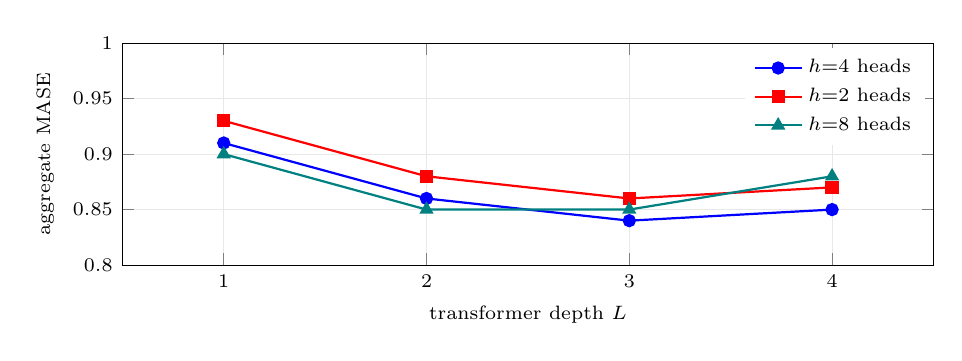
\begin{tikzpicture}
\begin{axis}[
    width=0.98\columnwidth,
    height=4.4cm,
    xlabel={transformer depth $L$},
    ylabel={aggregate MASE},
    xmin=0.5, xmax=4.5,
    ymin=0.80, ymax=1.00,
    xtick={1,2,3,4},
    legend style={font=\scriptsize, at={(0.99,0.98)}, anchor=north east, draw=none},
    tick label style={font=\scriptsize},
    label style={font=\scriptsize},
    grid=both,
    grid style={gray!18},
]
\addplot[blue, thick, mark=*, mark size=2pt] coordinates {(1,0.91)(2,0.86)(3,0.84)(4,0.85)};
\addlegendentry{$h{=}4$ heads}
\addplot[red, thick, mark=square*, mark size=2pt] coordinates {(1,0.93)(2,0.88)(3,0.86)(4,0.87)};
\addlegendentry{$h{=}2$ heads}
\addplot[teal, thick, mark=triangle*, mark size=2.2pt] coordinates {(1,0.90)(2,0.85)(3,0.85)(4,0.88)};
\addlegendentry{$h{=}8$ heads}
\end{axis}
\end{tikzpicture}
\caption{Effect of transformer depth $L$ and the number of heads $h$ on aggregate MASE. Two-to-three layers with four heads sit at the sweet spot; deeper models begin to overfit on the smaller datasets.}
\label{fig:heads_depth}
\end{figure}
